\section{Introduction}
\author{Kévin Moreau}


\begin{frame}
	\frametitle{Rappel du contexte}

	\begin{block}{L'entreprise Dynamease}
	 \begin{itemize}
      \item Start-up ;
	  \item Service de mise en communication contextualisée.
	 \end{itemize}
	\end{block}

    \begin{center}
	  \begin{figure}
        \includegraphics[scale=0.30]{images/dynamease.pdf}
	   \caption{Communication contextualisé}
	  \end{figure}
	\end{center}
\end{frame}

\begin{frame}
	\frametitle{Les clients Dynamease}

    \begin{description}
    	\item[Basic] Utilisation des fonctionnalités basiques des applications Dynamease;
    	\item[Avantage] Importation d'un calendrier externe de l'application;
    	\item[Privilège] Obtention d'un numéro Dynamease;
    	\item[Intégrale] Permet l'ajout d'employés.
    \end{description}

\end{frame}

\begin{frame}
	\frametitle{L'environnement Dynamease}

    \begin{center}
	  \begin{figure}
        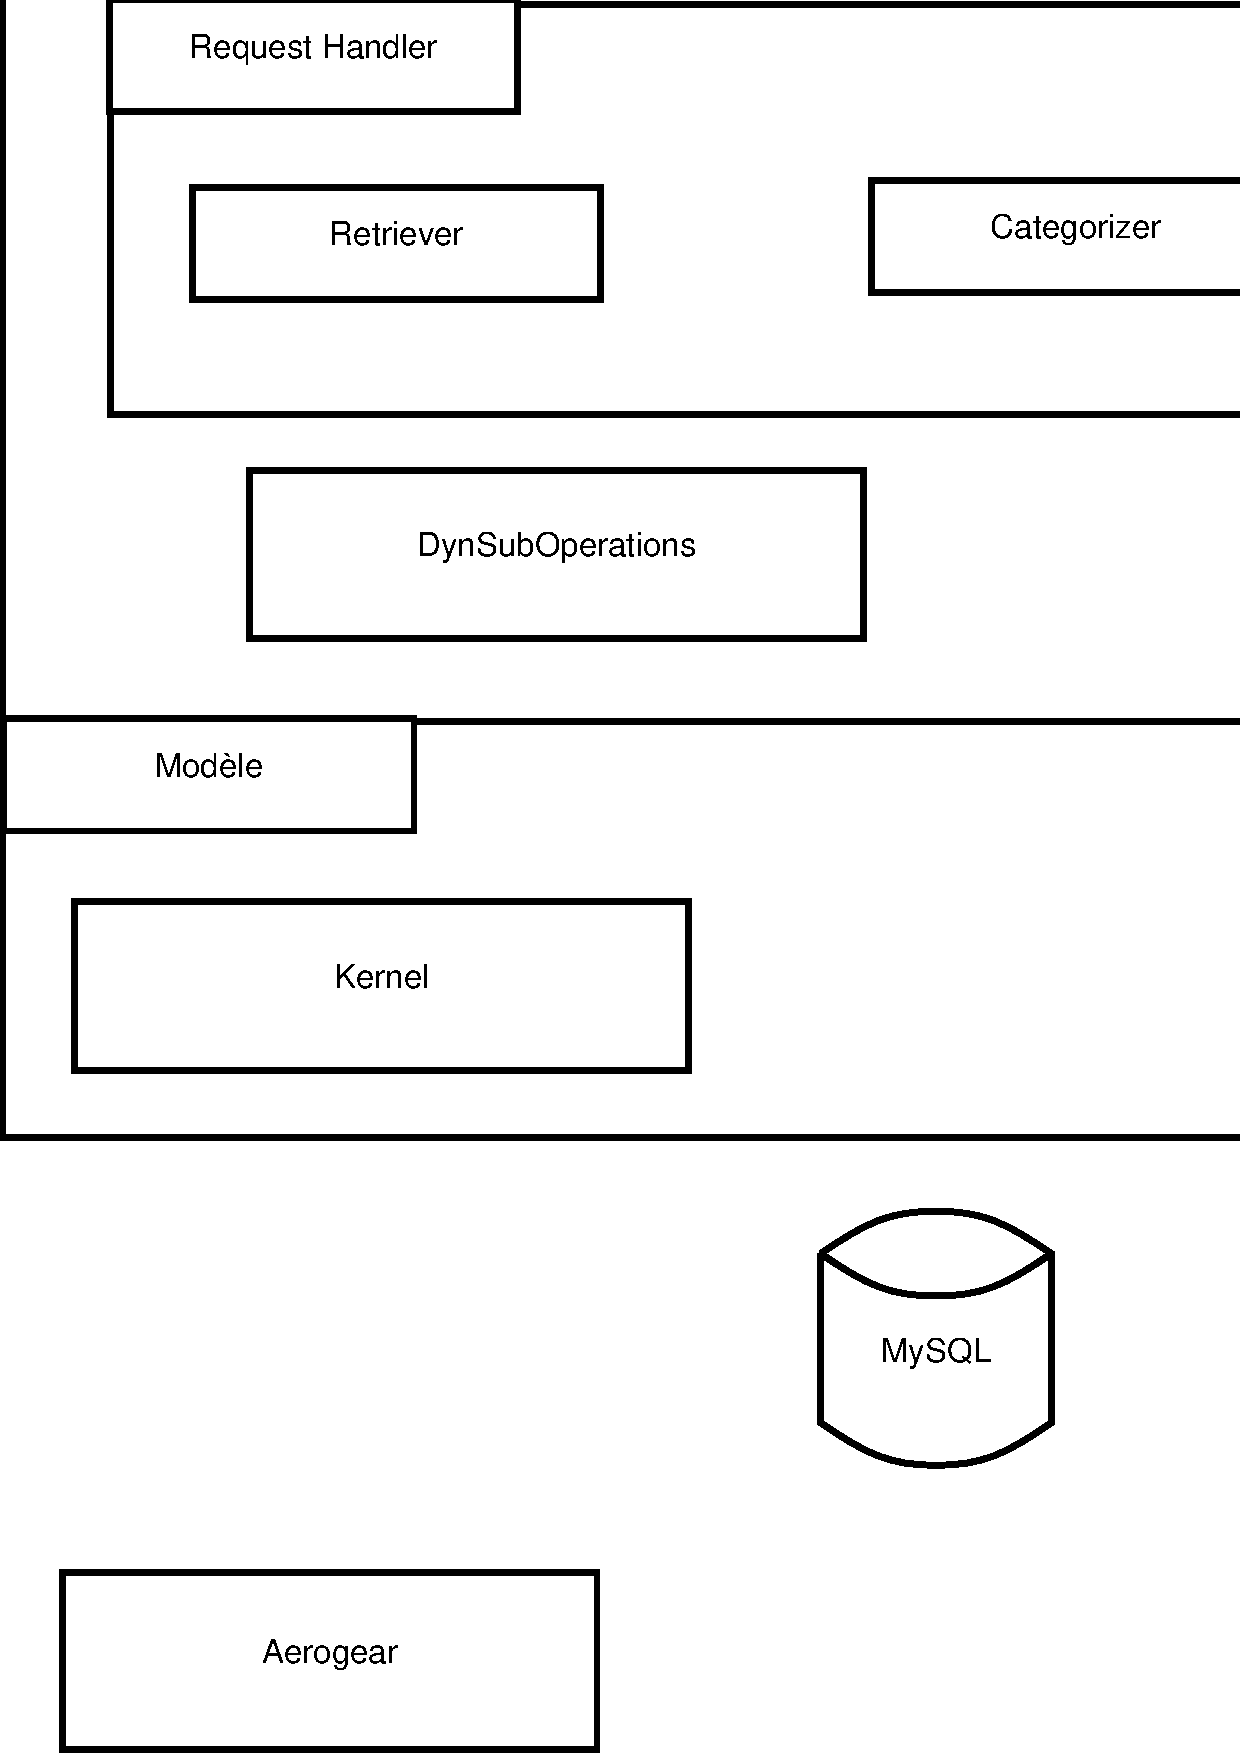
\includegraphics[scale=0.15]{images/composant.pdf}
	   \caption{Les différents composants de Dynamease}
	  \end{figure}
	\end{center}

\end{frame}

\begin{frame}
	\frametitle{Le sujet de mon stage}

	\begin{block}{Liste de mes objectifs}
	 \begin{itemize}
	  \item Améliorations des services clients et employés de Dynamease;
      \item Ajout de fonctionnalité pour les application téléphoniques;
	  \item Amélioration de la sécurité des communications entre les applications et le serveur Dynamease.
	 \end{itemize}
	\end{block}

\end{frame}


